\tableofcontents

\section*{Введение}
\addcontentsline{toc}{section}{Введение}

Поиск пути (англ. pathfinding) --- термин в информатике и искусственном интеллекте, который означает определение компьютерной программой наилучшего, оптимального маршрута между двумя точками \cite{wiki:pathfinding} (рисунок \ref{fig:pathfinding}).

\begin{figure}[ht]
    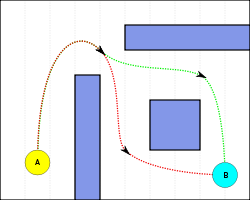
\includegraphics[width=.5\linewidth]{Figures/pathfinding.png}
    \caption{Путь между двумя точками}
    \label{fig:pathfinding}
\end{figure}

Большое распространение поиск пути получил в связи с развитием компьютерных игр, особенно стратегий реального времени, где игрок даёт задание игровым единицам двигаться через игровой уровень, содержащий препятствия. В стратегиях игровой уровень делится на тайлы (англ. tiles), которые действуют как \textbf{узлы} (англ. nodes) в алгоритме поиска пути \cite{wiki:pathfinding}.

Также алгоритм используется в 3D-шутерах, где взамен узлов используются так называемые \textbf{вэйпоинты} (англ. waypoints, дословно --- рус. точки пути). Вэйпоинты --- это нерегулярные и вручную установленные узлы, которые содержат информацию о том, к каким другим узлам возможно добраться от данного \cite{wiki:pathfinding}.

Так как игры становятся всё сложнее, то поиск пути также эволюционирует и развивается вместе с ними. В итоге существует ряд алгоритмов поиска пути, используемых не только для расчета в компьютерных играх, но также в технических системах зрения, промышленной автоматизации, области искусственного интеллекта и других областях.

По своей сути алгоритм поиска пути ищет на графе, начиная с одной (стартовой) точки и исследуя смежные узлы до тех пор, пока не будет достигнут узел назначения (конечный узел). Кроме того, в алгоритмы поиска пути в большинстве случаев заложена также цель найти самый короткий путь. Некоторые методы поиска на графе, такие как поиск в ширину, могут найти путь, если дано достаточно времени. Другие методы, которые ``исследуют'' граф, могут достичь точки назначения намного быстрее. Здесь можно привести аналогию с человеком, идущим через комнату. Человек может перед началом пути заранее исследовать все характеристики и препятствия в пространстве, вычислить оптимальный маршрут и только тогда начать непосредственное движение. В другом случае человек может сразу пойти в приблизительном или предполагаемом направлении цели и потом, уже во время пути, делать корректировки своего движения для избегания столкновений с препятствиями \cite{wiki:pathfinding}.

К самым известным и популярным алгоритмам поиска пути относятся такие алгоритмы \cite{wiki:pathfinding}:

\begin{itemize}
    \item алгоритм поиска A*;
    \item алгоритм Дейкстры;
    \item \textbf{волновой алгоритм};
    \item маршрутные алгоритмы;
    \item другие.
\end{itemize}

\section{Сущность алгоритмизации}

Понятие алгоритма является фундаментальной категорией математики и не может быть выражено через другие, более простые понятия, а рассматривается как нечто неопределяемое. Другими словами, единого определения алгоритма не существует, есть только разные подходы, описания этого понятия, причем, в полном соответствии с той областью знаний, где он применяется \cite{comp:algoritm}.

Алгоритм --- это строгая, четкая последовательность математических и логических операций, приводящая к решению задачи \cite{comp:algoritm}.

Алгоритмизация процессов в широком смысле --- это описание процессов на языке математических символов для получения алгоритма, отображающего элементарные акты процесса, их последовательность и взаимосвязь. Для построения алгоритма управления, например, необходимо к алгоритму, описывающему процесс функционирования системы, присоединить алгоритм определения оптимального решения или оптимальных значений параметров управления. В более узком смысле алгоритмизация --- это процедура поиска, разработки и описания алгоритма решения задачи \cite{comp:algoritm}.

Алгоритм должен обладать следующими свойствами \cite{comp:algoritm}:

\begin{itemize}
    \item детерминированностью;
    \item массовостью;
    \item результативностью;
    \item дискретностью;
    \item конечностью;
    \item корректностью.
\end{itemize}

Если разработанная последовательность действий не обладает хотя бы одним из перечисленных выше свойств, то она не может считаться алгоритмом.

\section{Типовые структуры алгоритмов}

Из многообразия всевозможных алгоритмов выделяются три основных типовых структуры \cite{comp:algoritm}:

\begin{itemize}
    \item линейная;
    \item разветвляющаяся;
    \item циклическая.
\end{itemize}

Конечно, отнести конкретный алгоритм к какой-либо из них полностью удается не часто, т.к. вычислительные задачи очень разные и по сути, и по методам решения. Однако, любой алгоритм, каким бы сложным он ни был, можно разбить на отдельные части, фрагменты, каждый из которых и является алгоритмом одной из перечисленных типовых структур. Каждая типовая структура имеет свои принципы построения, их необходимо знать и соблюдать при разработке своего алгоритма.

Линейными называются алгоритмы, в которых действия осуществляются последовательно друг за другом. Стандартная блок-схема линейного алгоритма приводится на рисунке \ref{fig:struct:linear} \cite{szci:struct}.

\begin{figure}[!ht]
    \subfloat[]{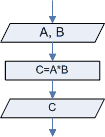
\includegraphics[width=.2\linewidth]{Figures/linear.png}\label{fig:struct:linear}}
    \qquad
    \subfloat[]{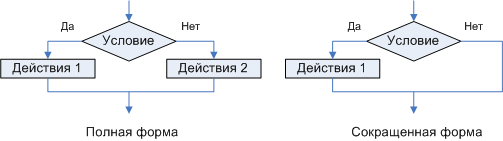
\includegraphics[width=.9\linewidth]{Figures/branching.png}\label{fig:struct:branching}}
    \qquad
    \subfloat[]{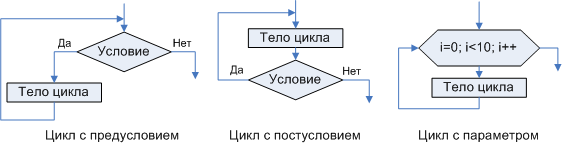
\includegraphics[width=.9\linewidth]{Figures/cyclical.png}\label{fig:struct:cyclical}}
    \caption{Базовые структуры алгоритмов: (а) линейные; (б) разветвляющиеся; (в) циклические}
    \label{fig:struct}
\end{figure}

Разветвляющимся называется алгоритм, в котором действие выполняется по одной из возможных ветвей решения задачи, в зависимости от выполнения условий. В отличие от линейных алгоритмов, в которых команды выполняются последовательно одна за другой, в разветвляющиеся алгоритмы входит условие, в зависимости от выполнения или невыполнения которого выполняется та или иная последовательность команд (действий).

В качестве условия в разветвляющемся алгоритме может быть использовано любое понятное исполнителю утверждение, которое может соблюдаться (быть истинно) или не соблюдаться (быть ложно). Такое утверждение может быть выражено как словами, так и формулой. Таким образом, алгоритм ветвления состоит из условия и двух последовательностей команд.

В зависимости от того, в обоих ветвях решения задачи находится последовательность команд или только в одной разветвляющиеся алгоритмы делятся на полные и не полные (рисунок \ref{fig:struct:branching}) \cite{szci:struct}.

Циклическим называется алгоритм, в котором некоторая часть операций (тело цикла — последовательность команд) выполняется многократно. Однако слово «многократно» не значит «до бесконечности». Организация циклов, никогда не приводящая к остановке в выполнении алгоритма, является нарушением требования его результативности — получения результата за конечное число шагов.

Если тело цикла расположено после проверки условий , то может случиться, что при определенных условиях тело цикла не выполнится ни разу. Такой вариант организации цикла, управляемый предусловием, называется циклом c предусловием.

Возможен другой случай, когда тело цикла выполняется по крайней мере один раз и будет повторяться до тех пор, пока не станет ложным условие. Такая организация цикла, когда его тело расположено перед проверкой условия, носит название цикла с постусловием.

Цикл с параметром является разновидностью цикла с предусловием. Особенностью данного типа цикла является то, что в нем имеется параметр, начальное значение которого задается в заголовке цикла, там же задается условие продолжения цикла и закон изменения параметра цикла. Механизм работы полностью соответствует циклу с предусловием, за исключением того, что после выполнения тела цикла происходит изменение параметра по указанному закону и только потом переход на проверку условия \cite{szci:struct}.

Стандартные блок-схемы циклических алгоритмов приведены на рисунке \ref{fig:struct:cyclical}.

\section{Методы разработки алгоритмов}
\label{sub:methods}

Составление алгоритмов решения задач - это работа творческая. Нет универсального способа, позволяющего без особого труда составлять любые алгоритмы. К сожалению, такого способа не существует, ведь жизненные ситуации и задачи так разнообразны и непредсказуемы! Если бы дело обстояло иначе, появилась бы реальная возможность автоматизировать сам процесс алгоритмизации, поручив его некоторому исполнителю - вероятно, очень высокоинтеллектуальному компьютерy \cite{comp:algoritm}.

Тем не менее, существуют некоторые рекомендации, касающиеся методики разработки алгоритмов. При решении простых задач можно воспользоваться определенной схемой. В большинстве случаев та или иная задача может быть решена несколькими численными методами. Выбор конкретного численного метода решения задачи обычно производится по следующим критериям:

\begin{itemize}
    \item обеспечение оптимального времени решения задачи;
    \item обеспечение оптимального использования имеющихся ресурсов (памяти);
    \item обеспечение требуемой точности вычислений;
    \item минимальные стоимостные затраты;
    \item возможность использования стандартных подпрограмм.
\end{itemize}

\textbf{Структурное программирование} - одна из популярных методик. Фундаментом структурного программирования является доказанная Бемом и Джекопини теорема о структурировании \cite{algorithm_theory}. Эта теорема устанавливает, что как бы сложна ни была задача, блок-схема соответствующей программы всегда может быть представлена с использованием весьма ограниченного числа элементарных управляющих структур (последовательность, ветвление, цикл).

Цель структурного программирования - выбор структуры программы путем расчленения исходной задачи на подзадачи. Программы должны иметь простую структуру. Сложные, запутанные программы, как правило, являются неработоспособными, а их тестирование требует больших затрат \cite{comp:algoritm}.

Разработка алгоритма, являясь четким логичным процессом, упрощается на каждом уровне шаг за шагом. Затем в процессе задействуется следующий метод алгоритмизации - \textbf{метод пошагового уточнения} (совершенствования).

Сначала задача рассматривается в целом, выделяются наиболее крупные ее части. Алгоритм, указывающий порядок выполнения этих частей, описывается в структурированной форме, не вдаваясь в мелкие детали. Затем от общей структуры переходят к описанию отдельных частей. Таким образом, разработка алгоритма состоит из последовательности шагов в направлении уточнения алгоритма.

Дальнейшим развитием, расширением структурного программирования является \textbf{модульное программирование}, идея которого состоит в том, что алгоритм может быть представлен в виде системы, совокупности отдельных модулей. Каждый модуль рассматривается как самостоятельная, относительно независимая программа, которая может содержать набор данных и функций, доступных только из этого модуля.

Модульное программирование позволяет значительно ускорить процесс засчет привлечения к работе нескольких специалистов сразу, доверив каждому разработку отдельного модуля. Кроме того, модульное программирование предполагает возможность использования заранее разработанных стандартных программ (т.н. библиотек стандартных подпрограмм).

На этапе проектирования алгоритма решения сложной задачи, состоящей из нескольких подзадач,  используют два подхода: нисходящий и восходящий.

При нисходящем проектировании вначале проектируются функции управляющей программы - драйвера. Затем более подробно представляют каждую подзадачу и разрабатывают другие модули. При нисходящем проектировании на каждом шаге функционирование модуля описывается с помощью ссылок на последующие, более подробные шаги.

При восходящем проектировании  вначале проектируют программы низшего уровня, иногда в виде самостоятельных подпрограмм. Затем на каждом шаге разрабатываются модули более высокого уровня \cite{comp:algoritm}.

Существует также несколько общих алгоритмических методов решения очень сложных задач. Более подробно ознакомиться с некоторыми из них можно в \cite{gudman:alg_coding} (методы частных целей, подъема и отрабатывания назад, метод ветвей и границ и др.).

\section{Волновой алгоритм}

Существует множество алгоритмов поиска пути со своими преимуществами и недостатками. Многие алгоритмы несовершенны и позволяют завести себя в тупик (рисунок \ref{fig:bumper}). Волновой алгоритм отличается тем, что он позволяет найти путь в \textbf{любом} лабиринте с \textbf{любым} количеством препятствий. Его недостатком является то, что он требует огромных затрат памяти.

\begin{figure}[ht]
    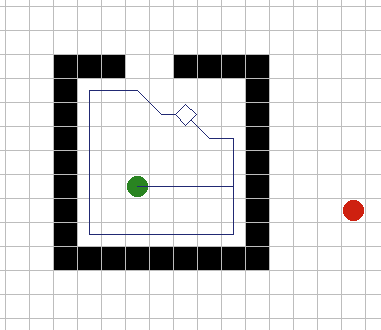
\includegraphics[width=.6\linewidth]{Figures/bumper.png}
    \caption{Несовершенный алгоритм}
    \label{fig:bumper}
\end{figure}

Алгоритм волновой трассировки (волновой алгоритм, алгоритм Ли) --- алгоритм поиска пути, алгоритм поиска кратчайшего пути на планарном графе. Принадлежит к алгоритмам, основанным на методах поиска в ширину \cite{wiki:li}.

В основном используется при компьютерной трассировке (разводке) печатных плат, соединительных проводников на поверхности микросхем. Другое применение волнового алгоритма --- поиск кратчайшего расстояния на карте в компьютерных стратегических играх \cite{wiki:li} (например, прохождение лабиринта).

Волновой алгоритм в контексте поиска пути в лабиринте был предложен Э. Ф. Муром. Ли независимо открыл этот же алгоритм при формализации алгоритмов трассировки печатных плат в 1961 году \cite{wiki:li}.

Плюс алгоритма в том, что он позволяет найти путь в любом лабиринте (при условии, что путь существует). Но главный недостаток этого алгоритма в том, что при построении трассы требуется большой объем памяти \cite{suv:li}.

Работа алгоритма включает в себя три этапа: \textbf{инициализацию}, \textbf{распространение волны} и \textbf{восстановление пути} \cite{wiki:li}.

Во время \textbf{инициализации} строится образ множества ячеек обрабатываемого поля, каждой ячейке приписываются атрибуты проходимости/непроходимости, запоминаются стартовая и финишная ячейки.

Далее от стартовой ячейки порождается шаг в соседнюю ячейку, при этом проверяется, проходима ли она, и не принадлежит ли ранее меченной в пути ячейке.

Соседние ячейки принято классифицировать двояко в смысле окрестности Мура и окрестности фон Неймана, отличающийся тем, что в окрестности фон Неймана соседними ячейками считаются только 4 ячейки по вертикали и горизонтали, в окрестности Мура --- все 8 ячеек, включая диагональные (рисунок \ref{fig:mooreneim}).

\begin{figure}[ht]
    \subfloat[]{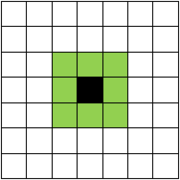
\includegraphics[width=.25\linewidth]{Figures/moore.png}}
    \qquad
    \subfloat[]{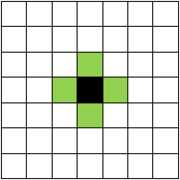
\includegraphics[width=.25\linewidth]{Figures/neim.png}}
    \caption{Окрестности (а) Мура; (б) фон Неймана}
    \label{fig:mooreneim}
\end{figure}

При выполнении условий проходимости и непринадлежности её к ранее помеченным в пути ячейкам, в атрибут ячейки записывается число, равное количеству шагов от стартовой ячейки. Каждая ячейка, меченая числом шагов от стартовой ячейки, становится стартовой и из нее порождаются очередные шаги в соседние ячейки. Очевидно, что при таком переборе будет найден путь от начальной ячейки к конечной, либо очередной шаг из любой порождённой в пути ячейки будет невозможен. Весь этот процесс и является \textbf{распространением волны} (рисунок \ref{fig:steps} \cite{byte:li}).

\begin{figure}[ht]
    \subfloat[]{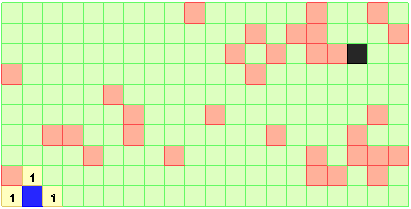
\includegraphics[width=.4\linewidth]{Figures/first.png}}
    \qquad
    \subfloat[]{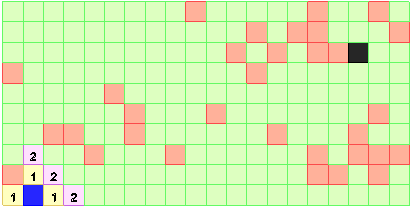
\includegraphics[width=.4\linewidth]{Figures/second.png}}
    \qquad
    \subfloat[]{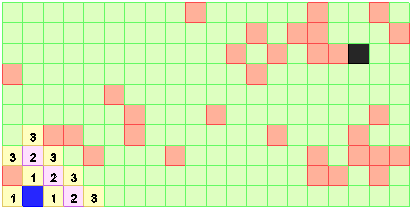
\includegraphics[width=.4\linewidth]{Figures/third.png}}
    \qquad
    \subfloat[]{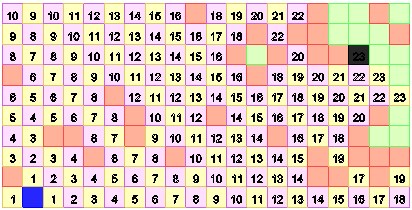
\includegraphics[width=.4\linewidth]{Figures/last.png}}
    \caption{Распространение волны (а) первый шаг; (б) второй шаг; (в) третий шаг; (г) последний шаг}
    \label{fig:steps}
\end{figure}

\textbf{Восстановление пути} происходит в обратном направлении: при выборе ячейки от финишной ячейки к стартовой на каждом шаге выбирается ячейка, имеющая атрибут расстояния от стартовой на единицу меньше текущей ячейки. Очевидно, что таким образом находится кратчайший путь между парой заданных ячеек \cite{wiki:li,byte:li} (рисунок \ref{fig:trace}).

\begin{figure}[ht]
    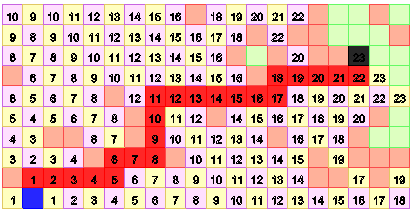
\includegraphics[width=.7\linewidth]{Figures/trace.png}
    \caption{Формирование пути}
    \label{fig:trace}
\end{figure}

\section*{Заключение}
\addcontentsline{toc}{section}{Заключение}

Волновой алгоритм поиска пути, или алгоритм Ли, черезвычайно эффективен, если нам необходимо найти путь в каком-либо сложном лабиринте и нет времени анализировать сам лабиринт. При возможности прохождения из начальной точки в конечную, алгоритм Ли просчитает кратчайший путь почти без проблем. Единственной проблемой остается ресурсоемкость алгоритма. Для нахождения пути в достаточно больших лабиринтах необходимо большое количество памяти и достаточно мощные ресурсы. С учетом технологического прогресса на сегодняшний день это не проблема, однако это нерационально.

Если есть время анализировать лабиринт, можно подобрать или спроектировать специализированный алгоритм, который управится с расчетами быстрее и задействует меньше ресурсов. Однако как говорилось в главе \ref{sub:methods}, конструирование алгоритма творческий и достаточно сложный процесс, поэтому имеет смысл довериться волновому алгоритму при наличии необходимых ресурсов.

\clearpage
\bibliography{../web,../books}
